\documentclass[10pt,handout]{beamer}
\usetheme{Rochester}
\usepackage[utf8]{inputenc}
\usepackage{amsmath}
\usepackage{amsfonts}
\usepackage{amssymb}
%\setbeamertemplate{frametitle}[default][center]
\setbeamercolor{page number in head/foot}{fg=black}
\setbeamerfont{page number in head/foot}{size=\small}
\usepackage{xcolor}
\setbeamertemplate{footline}[page number]
%\beamertemplatenavigationsymbolsempty
%\setbeamertemplate{footline}[page number]
%\setbeamertemplate{footline}[frame number]
%\usepackage{siunitx}
\author{Justin Anguiano, Margaret Lazarovitz}
\title{\textcolor{red}{Classifying Charged Particles} from High Energy Collisions at the \textcolor{red}{L}arge \textcolor{red}{H}adron \textcolor{red}{C}ollider }


%\setbeamercovered{transparent} 
%\setbeamertemplate{navigation symbols}{} 
%\logo{} 
\institute{University of Kansas} 
\date{\today} 
%\subject{} 
\begin{document}

%\begin{frame}
%\titlepage
%\end{frame}






\begin{frame}{Our Approach}
Deep neural network with two kinds of predictions:
\begin{itemize}
\item Binary classification: muon vs. everything else
\item Multi-class classification: muon, pion, kaon, proton, unmatched
\end{itemize}
\end{frame}

\begin{frame}{Data Preparation}
\begin{itemize}
\item Taking data from ROOT trees and converted it to pandas DataFrames
\item Evenly sampled among classes from different MC generated processes
\begin{itemize}
\item Each process produces kinematically different muons
\item Muons also have different origins
\end{itemize}
\item One-hot encoded the classes for categorical output
\item Normalized data
\end{itemize}
\end{frame}

\begin{frame}{Network Input}
\begin{itemize}
\item Minimal model: good muon variables (cut-based benchmark)
\item Complex model: energy, position, track information (MVA benchmark)
\item Custom: combination of the two
\end{itemize}
\end{frame}



\begin{frame}{Network Architecture}
\begin{itemize}
\item 4 hidden layers
\item 128 neurons/layer
\item ReLU activation
\item Softmax activation on last layer
\item Adam optimizer
\item Categorical cross entropy loss
\end{itemize}
\end{frame}

\begin{frame}{Training Stats}
\begin{itemize}
\item 35/65 test/training split
\item 10/90 validation/training split
\item 100 epochs
\item 256 batch size
\item Accuracy, loss, efficiency, and ROC curve
\end{itemize}
\end{frame}


\begin{frame}{Results: Binary Classifier}
Network statistics \\
\quad \quad
\begin{columns}
\begin{column}{0.3\textwidth}
Training
\begin{itemize}
\small
\item Accuracy: 0.9916
\item Loss: 0.0249
\end{itemize}
\end{column}
\begin{column}{0.3\textwidth}
Validation
\begin{itemize}
\small
\item Accuracy: 0.9247
\item Loss: 0.95241
\end{itemize}
\end{column}
\begin{column}{0.3\textwidth}
Test
\begin{itemize}
\small
\item Accuracy: 0.9235
\item Loss: 0.4939
\end{itemize}
\end{column}
\end{columns}
\end{frame}


\begin{frame}{Results: Binary Classifier}
Muon Classification \\
\quad \quad
\begin{itemize}
\item Recall (Correct ID rate): 99.9869\%
\item Purity (MisID rate): 9.2677\%
\end{itemize}
\quad \quad \\
Recall = $\frac{TP}{TP+FN}$ \\
\quad \\
Purity = $\frac{FP}{TP+FP}$
\end{frame}


\begin{frame}{Results: Multiclass Classifier}
Network statistics \\
\quad \quad
\begin{columns}
\begin{column}{0.3\textwidth}
Training
\begin{itemize}
\small
\item Accuracy: 0.9303
\item Loss: 0.1925
\end{itemize}
\end{column}
\begin{column}{0.3\textwidth}
Validation
\begin{itemize}
\small
\item Accuracy: 0.6804
\item Loss: 1.7296
\end{itemize}
\end{column}
\begin{column}{0.3\textwidth}
Test
\begin{itemize}
\small
\item Accuracy: 0.6797
\item Loss: 1.6903
\end{itemize}
\end{column}
\end{columns}
\end{frame}

\begin{frame}{Results: Multiclass Classifier}
\begin{columns}
\begin{column}{0.5\textwidth}
Muon Classification
\begin{itemize}
\item Recall (Correct ID rate): 
\item Purity (MisID rate): 
\end{itemize}
Pion Classification
\begin{itemize}
\item Recall: 
\item Purity: 
\end{itemize}
\end{column}
\begin{column}{0.5\textwidth}
Kaon Classification
\begin{itemize}
\item Recall: 
\item Purity: 
\end{itemize}
Proton Classification
\begin{itemize}
\item Recall: 
\item Purity: 
\end{itemize}
\end{column}
\end{columns}

\quad  \\
\quad  \\
Recall = $\frac{TP}{TP+FN}$ \\
\quad \\
Purity = $\frac{FP}{TP+FP}$
\end{frame}

\begin{frame}{Baseline Model}
\begin{itemize}
\item Cut-based ID - uses cuts on a few key variables
\item Soft MVA - gradient boosted regression forest
\item Looked at 3 different samples: DY+Jets, TT+Jets, and QCD
\item Efficiency $\epsilon$ = \# true muons that pass ID/\# true muons
\end{itemize}
\end{frame}




\begin{frame}{Baseline Model Performances}
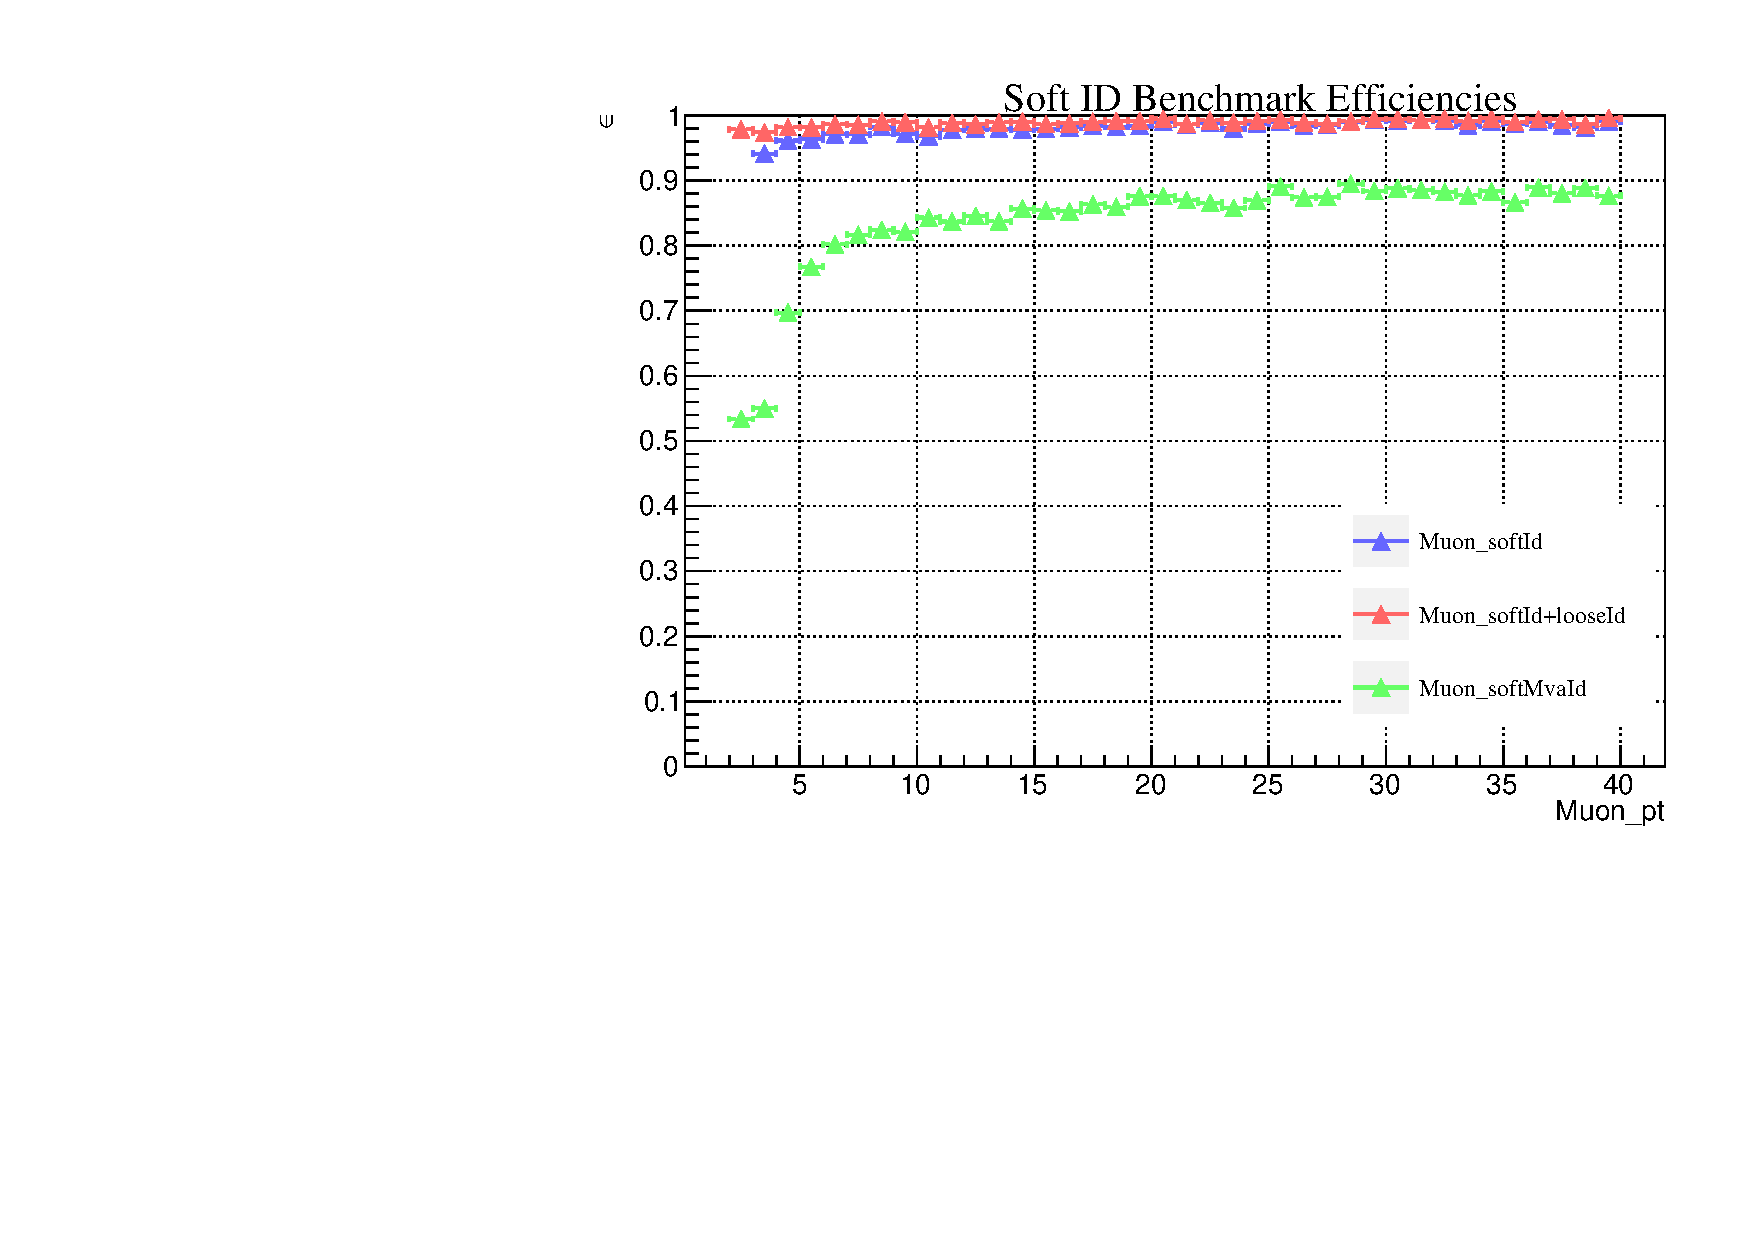
\includegraphics[scale=.5]{benchmarkEfficiency_TTjets.pdf}

$\epsilon$ = \# true muons that pass ID/\# true muons
\end{frame}


\begin{frame}{Baseline Model Performances}
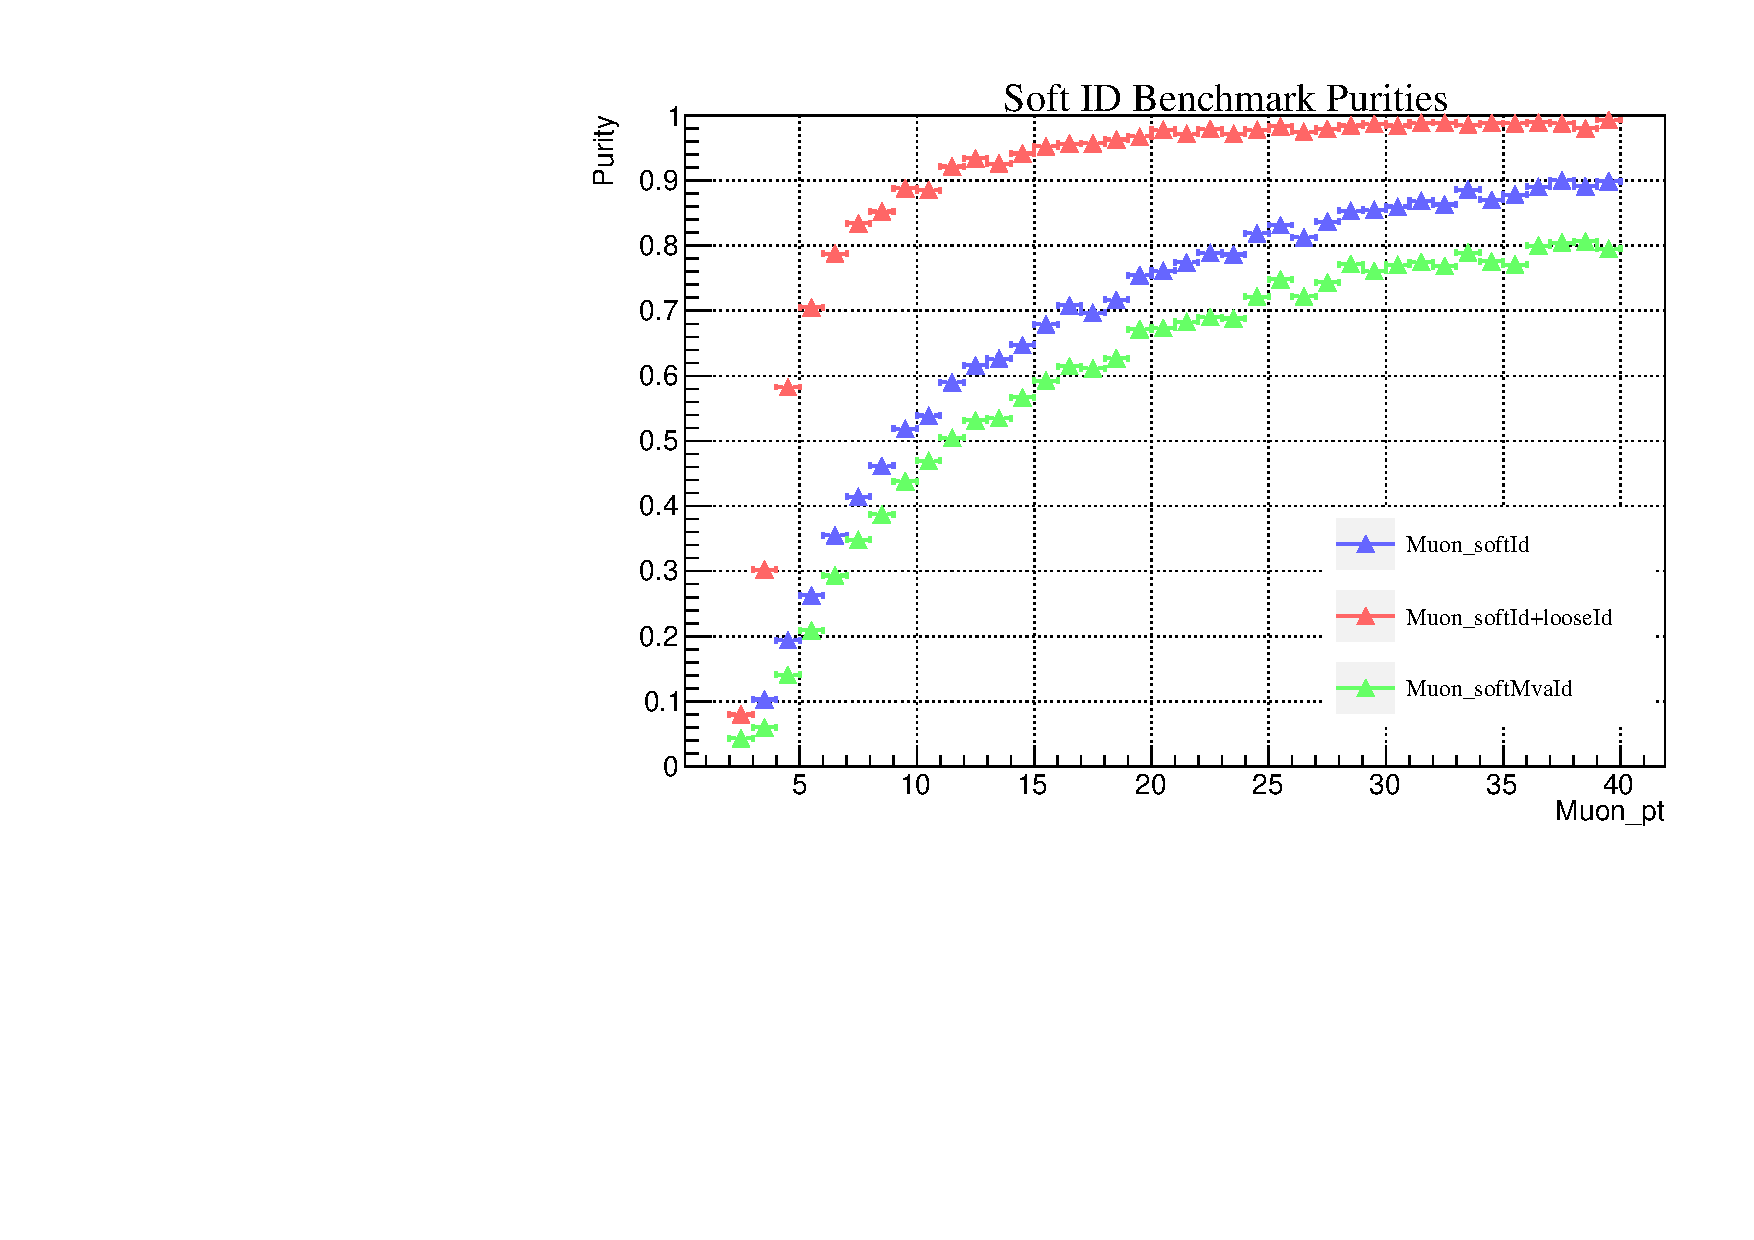
\includegraphics[scale=.5]{benchmarkPurity_TTjets.pdf}

Purity = \# true muons that pass ID/ \#reconstructed muons
\end{frame}

\begin{frame}{Summary}
Project Repository: \url{https://github.com/Jphsx/KUSoftMVA}
\end{frame}

\begin{frame}{backup}
\end{frame}






\begin{frame}{Baseline Model Performances}
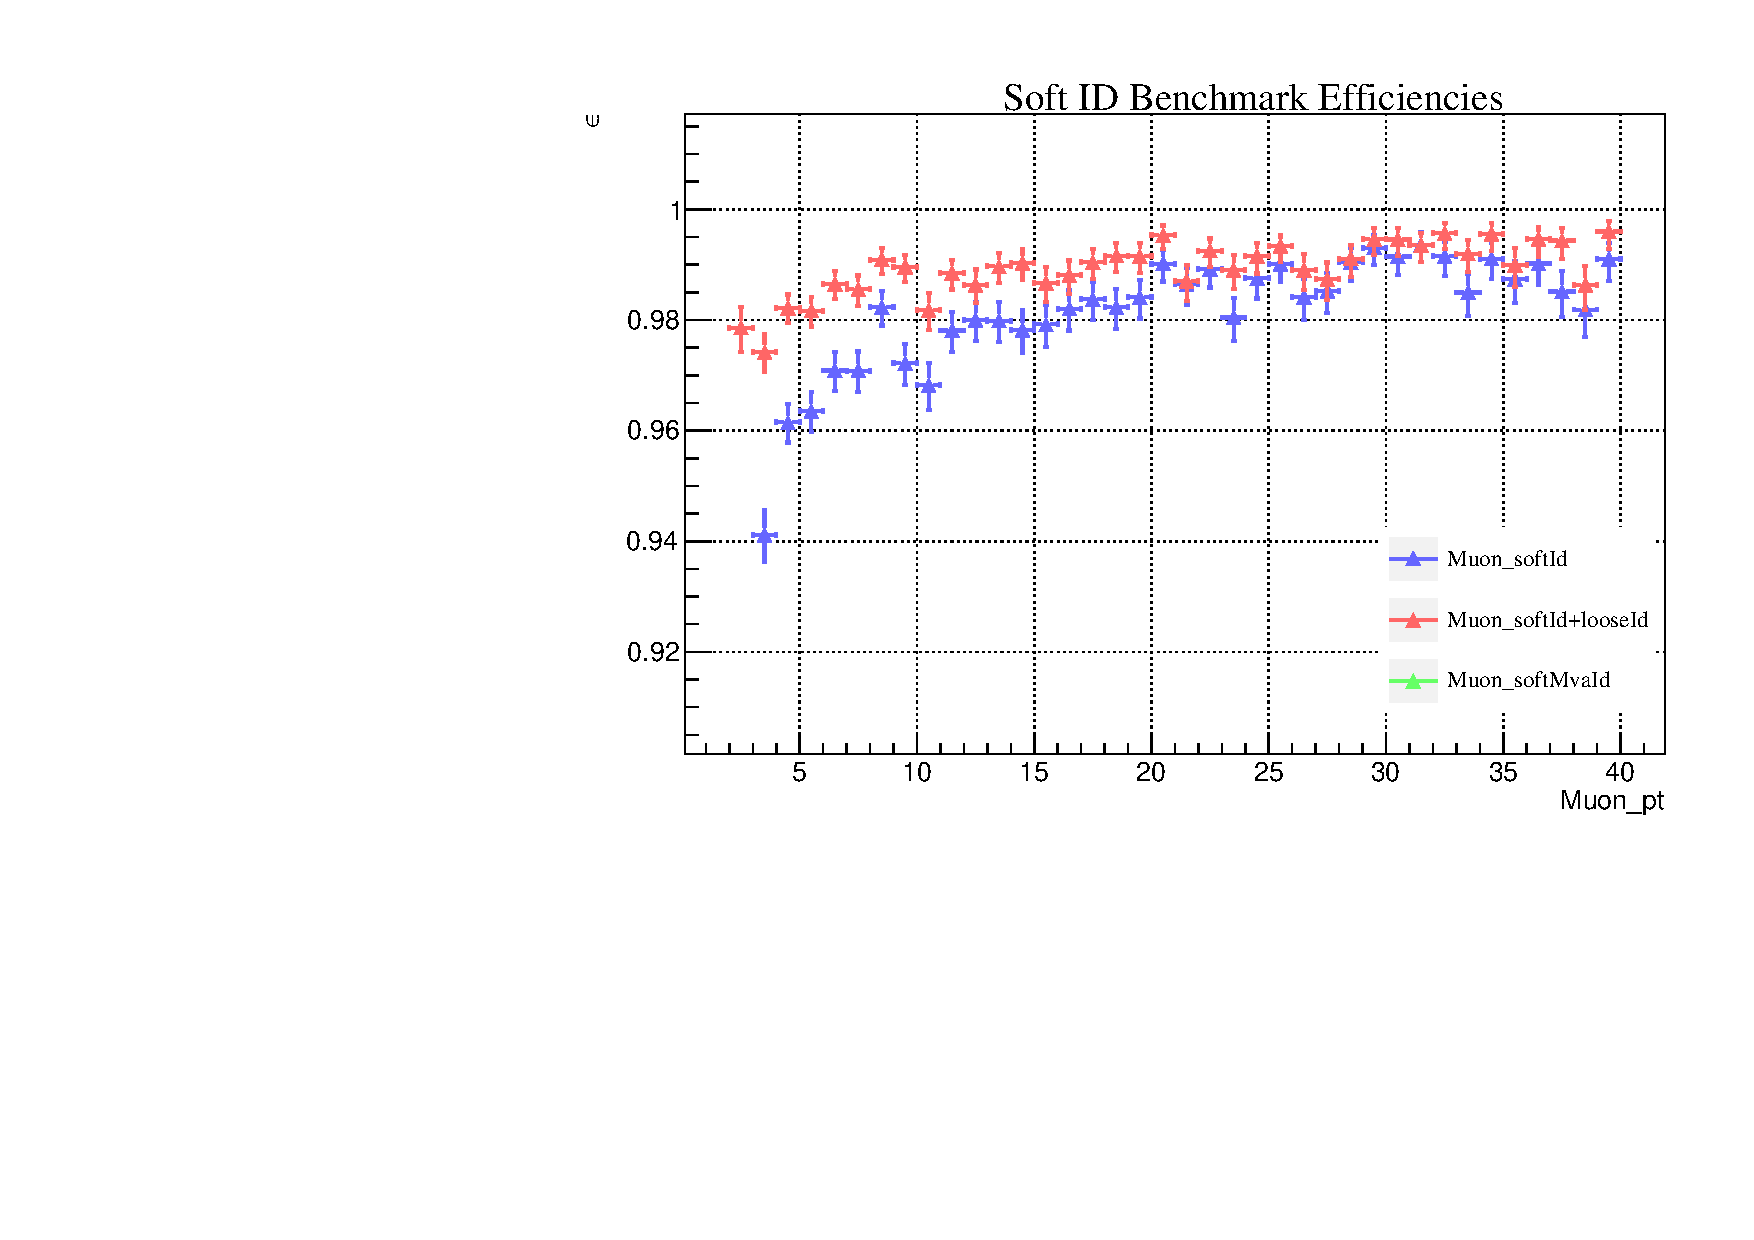
\includegraphics[scale=.5]{benchmarkEfficiency_TTjetszoomed.pdf}

$\epsilon$ = \# true muons that pass ID/\# true muons
\end{frame}












\end{document}